% A simple template for LaTeX documents
% 
% To produce pdf run:
%   $ pdflatex paper.tex 
%

\documentclass[12pt]{article}

% Begin paragraphs with new line
\usepackage{parskip}  

% Change margin size
\usepackage[margin=1in]{geometry}   

% Graphics Example:  (PDF's make for good plots)
\usepackage{graphicx}               
% \centerline{\includegraphics{figure.pdf}}

% Allows hyperlinks
\usepackage{hyperref}

% Blocks of code
\usepackage{listings}
\lstset{basicstyle=\ttfamily, title=\lstname}
% Insert code like this. replace `plot.R` with file name.
% \lstinputlisting{plot.R}

% Supports proof environment
\usepackage{amsthm}

% Allows writing \implies and align*
\usepackage{amsmath}

% Allows mathbb{R}
\usepackage{amsfonts}


%%%%%%%%%%%%%%%%%%%%%%%%%%%%%%%%%%%%%%%%%%%%%%%%%%%%%%%%%%%%
\begin{document}

\title{US Korea Exchange Rates \\ STA206 Final Project}
\date{December 15, 2014}
\author{Clark Fitzgerald clarkfitzg@gmail.com \\ 
        Amy Kim atykim@ucdavis.edu}

\maketitle

\begin{abstract}

    We analyze the exchange rate between the United States and South Korea
    (hereafter Korea) using monthly country level economic data and find
    that ratios of economic indicators are useful in confirming economic
    reasoning about the relative strengths of the two national economies.

\end{abstract}

\section{Introduction}

\subsection{Background}

In today's highly connected global society people and money move between
countries. The exchange rates between countries determine the relative
value of that money.

We analyze data on exchange rate between the US and Korea from 1999 to
2014. In 1997 the IMF crisis in Korea perturbed the economic indicators,
but they have been mostly stable since 1999.

\subsection{Questions}

\begin{enumerate}

    \item How do exchange rates behave?

    \item Can we predict the exchange rate between two countries?  

    \item When is the best time to exchange currency from Korean Won
        to US Dollar or vice versa?  

    \item Can we find a linear relationship
        that can be applied over other countries' currency? 

\end{enumerate}

\subsection{Motivation}

Sometimes it's necessary to transfer funds between countries. This is true
for both individuals, families, and organizations. The exchange rate can
vary substantially over time. For example, in
Figure~\ref{fig:exchange_rate} we observe the exchange rate between Korea
and the US varying between 900 and 1400 Korean Won per US Dollar. A quick
calculation on this data 
implies that during this period a fixed amount of Korean currency 
could have been worth \$100,000 or \$158,000, depending on when it was  
exchanged. 

Hence if one has a significant amount of capital to move from
one country to another and some flexibility around the timing then it makes
sense to do it when the exchange rates
are favorable for the transfer. For example, you may want to sell a
house in Korea and put that money towards a house in the US.

\subsection{Data}

We use data from Quandl.com, a service that provides clean, documented
data from a wide variety of sources including the US Federal Reserve,
World Bank, and the National Bank of Korea. 
{\tt Exchange rate} between Korean Won and US dollar is the primary $Y$
variable.

For each country we will examine the following variables:

\begin{itemize}
    \item {\tt gdp} The gross domestic product. Units: USD Million
    \item {\tt unemployment rate} The percentage of the labor force who are unemployed and actively seeking work. Units: Percent (monthly)
    \item {\tt exports} The total value of the goods and services
produced domestically and purchased by foreign entities. Units: USD Million (Monthly)
    \item {\tt imports} The total value of a country's imports of physical goods and payments to foreigners for services like shipping and tourism. Units: USD Million (Monthly)
    \item {\tt interest rate} The monthly average of the central bank policy rate. This is the interest rate the central bank charges on loans to commercial banks. Units: Percent (Monthly)
    \item {\tt inflation rate} The growth rate of the prices. (Monthly)
    \item {\tt consumer produce index} The Consumer Price Index (CPI) is a measure of inflation related to the cost of living. Units: Index Points 2010=100, NSA (Monthly)
    \item {\tt debt} The total amount of public and private debt owned by foreign creditors. Units: USD Million Current Prices, NSA (quarterly)
    \item {\tt gdp deflator} The relative difference between the real and nominal GDPs. Units: Index Points NSA
    \item {\tt goverment spending} The yearly expenditure of the federal
        government. Units: local currency
\end{itemize}

\section{Methods and Results}

\subsection{Dynamic Data}

The data used in this analysis is unusual- it's generated dynamically from
live, high quality sources, and is self updating. The data is loaded directly from Quandl using a REST (Representational 
State Transfer) web API (Application programming interface), and then
cached locally, limiting network dependence.
Using this service makes it easy to repeat the analysis in the future, or conduct similar analyses between
different countries.

Through a little engineering the data analysis process
can be made transparent, automated, extensible, and fully reproducible.
For more information on the techniques please refer to the section on
Reproducibility in the appendix.

\subsection{Exploratory Data Analysis}

We started out with some general summary statistics and plotting. The first
issue was missing data, which we had anticipated. While most of the
variables were reported monthly, some were reported on a quarterly or
annual basis. (Figure~\ref{fig:na_plot_KOR})
Our simple approach for dealing with this was to
make a plot of these variables over time.
If they are approximately linear then we could 
linearly interpolate with respect to time. The scaled plots 
Figure~\ref{fig:na_plot_KOR} and
Figure~\ref{fig:na_plot_USA} do appear to be mostly linear, so we interpolated. 
In this plots one can observe that \texttt{debt\_USA} is decreasing; this is
because \texttt{debt} carries a sign.

When beginning this project we knew that the time dependency and
multicollinearity would be the
biggest obstacles, since in this case the assumption that the errors
$\epsilon_i \sim N(0, \sigma^2)$ does not hold.
Figure~\ref{fig:scatterplot} shows what the original data looks like.
We observe clear patterns emerging, with some even approaching a
continuous mathematical functional relationship- ie the patterns
between \texttt{gdp}, \texttt{gdp\_deflator}, and \texttt{debt} for Korea.
Figure~\ref{fig:correlation} shows a histogram of all the pairwise sample
correlations for the original data set- they are highly correlated. In
fact, 30 \% of the columns have absolute sample correlation greater than 0.9.

Our first approach for overcoming this time dependence was to create a new
data frame from the original data by taking the difference between each
subsequent row (monthly difference). 
More formally, if our original design matrix $X$ is $n
\times p$ then we can define a new $n - 1 \times p$ matrix $\tilde{X}$ by
setting
\[
    \tilde{X_{i,*}} = X_{(i + 1), *} - X_{i, *}
\]
for $i = 1, 2, \dots, n-1$ where $X_{i, *}$ represents the $i$th row of
$X$.

As can be observed in Figure~\ref{fig:diff_scatterplot},
this approach did indeed eliminate the most obvious patterns, but 
at the expense of interpretability. We attempted regression on this
transformed data, but were unsuccessful.

\subsection{Ratios}

Because exchange rate is a ratio of Korean currency / US dollar we decided
to make transformed variables consisting of the Korean economic indicator
divided by the corresponding US indicator. We also included
\texttt{inflation} untransformed since the US has value 0 for some time
periods, meaning that this transformation is not defined.
\texttt{Date} was intentionally left out of the model in order
to be able to interpret the model in terms of the other parametrs. However,
the effects of time are still present through the variables that are linear
over time.

\subsection{Analysis}

Our first step when fitting the model was to separate the data into
training and validation sets. We checked to make sure that the variables
looked approximately the same in both training and validation sets.

We used forward stepwise selection to choose a model. 
Based on the criteria from the output of the \texttt{leaps regsubsets}
in the appendix we chose to explore a
model with an intercept and 5 predictor variables. The one with 5
predictors had the lowest BIC of all the models, and the Mallow's CP at
5.39 was significantly better than the model with 4 predictors which had a
CP value of 13.91. Since 5.39 is close to 5 and 13.91 is pretty far from 4
we conclude that the model with 5 variables is correct, meaning that it has
little bias.

The variables under further investigation are:
\texttt{gdp}, \texttt{interest\_rate}, \texttt{inflation\_KOR}, 
\texttt{inflation\_USA}, and \texttt{govspending}. (Model 1)

The box - cox transformation in figure~\ref{fig:boxcox} suggests a
transformation of $1 / x^2$, but this is extreme and is due to the
outliers. Instead we used the multiplicative inverse transformation on the
\texttt{exchange\_rate}, which has the appealing property of maintaining
interpretability; instead of Korean Won / USD we have USD / Korean Won.

The outliers can be readily detected in the diagnostic plots 
figure~\ref{fig:cooks}. We see
that the points 113 and 117 are the primary outlying cases, which have
absolute DFFIT values of 1.16 and 0.89. This is much bigger than the cutoff
of $2 \sqrt{p / n} = 0.445$. Cook's distance is large as well.
Looking up the
corresponding dates reveals that these are the points occuring during
October 2008 and February 2009, during the subprime mortgage crisis
which shook the global economy. There are no points between 113 and 117
because the test train split didn't select them. In the validation set we
discovered similar results for this period(114, 118). The subprime mortgage
crisis is the reason that they are outliers. So, we took off the outliers
from our data set to get model 1 fit~\ref{m1:train}. We also had trouble
with recent dates having large leverage values of around 0.16, which is
greater than the threshold of $2 * p / n = 0.08$.

When checking this final model with the validation set, then the
\texttt{govspending} variable is not
significant (P-value:0.312)~\ref{m1:test}. The added-variable plot in
figure~\ref{fig:added} indicates \texttt{govspending} contains no
additional information useful for predicting (1/exchage\_rate) beyond the
other variable, so it is not helpful to add \texttt{govspending} to our
model. Thus, we decide the our final variables are \texttt{gdp},
\texttt{interest\_rate}, \texttt{inflation\_KOR}, and
\texttt{inflation\_USA}~\ref{finalmodel}. The corresponding equation is:

$\frac{1}{exchange\_rate} = 3.868323e^{-4} + 9.692157e^{-3} * gdp
-1.289123e^{-5} *interest\_rate -2.573026e^{-5} * inflation\_KOR +
2.135945e^{-5}  * inflation\_USA$ 

For this model we have $R^2 = 0.85, MSE = 1.28^{-9}$.

\subsection{Centering and Signs}

The model above is difficult to interpret, so we decided to center the data
to minimize multicollinearity and instead focus on the sign of the
coefficients. After a
similar analysis process we found that the final model
for the centered data has the same variables as well as \texttt{exports}.
The interesting part here were again the outliers, which this time also included
a point from the 2000 financial crisis (see \ref{centered} in the appendix). This fit came out
quite well, and the corresponding diagnostic plots can be seen in 
Figure \ref{fig:final_residual}.

We used Bonferroni's method to construct simultaneous 95\% confidence intervals
for each of the 5 variables selected in the centered model, producing the
following intervals:

\begin{table}[ht]
\centering
\begin{tabular}{rrr}
  \hline
 & lower & upper \\
  \hline
  gdp & -0.80 & -0.57 \\
  exports & -0.37 & -0.13 \\
  interest\_rate & 0.51 & 0.68 \\
  inflation\_KOR & 0.22 & 0.35 \\
  inflation\_USA & -0.37 & -0.22 \\
   \hline
\end{tabular}
\end{table}

\section{Conclusions and Discussion}

Let $Y$ be the exchange rate of Korean Won per US Dollar. Let $G, E, R, I$
represent the value of GDP, exports, interest rate, and inflation, respectively.
Let $X_K$ be the values for Korea and $X_{US}$ be the ones for the US. Let
$c_i$ be a nonnegative scalar for scaling.
The final model becomes

\[
    Y = Intercept -c_1 \frac{G_{K}}{G_{US}}
    -c_2 \frac{E_{K}}{E_{US}}
    +c_3 \frac{R_{K}}{R_{US}}
    +c_4I_{K} - c_5 I_{US} + \epsilon.
\]

The 95\% confidence interval does not include 0 for any of these variables,
so we are 95\% confident that the signs of the coefficients are correct. Since the predictor variables
are scaled or ratios they are unitless. Now the model has a
natural interpretation. Suppose that the Korean economy grows while the US
economy remains stagnant. This should be associated with a decreasing
exchange rate, because
the Korean Won will have more value relative to the US Dollar.
From our model we can infer the following:

\begin{enumerate}
    \item The negative coefficient of $\frac{G_{K}}{G_{US}}$ means that as
        the GDP of Korea increases relative to that of the US, the exchange
        rate decreases. 
    \item The negative coefficient of $\frac{E_{K}}{E_{US}}$ means that if
        Korea increases its exports relative to the US, the exchange rate
        decreases.
    \item The positive coefficient of $I_K$ means that the exchange rate
        increases as the inflation in Korea gets larger. This is a direct
        relation that we would expect.
    \item The negative coefficient of $I_{US}$ means that the exchange rate
        decreases as the inflation in the US gets larger.
\end{enumerate}

Common sense and economic reasoning tells us that all of these statements should be
true. The data and analysis confirm our intuition. Perhaps with the use of
time series techniques this analysis could be extended.

Now we return to our original questions. The results of this analysis 
suggest a reasonable course of action if you want to exchange your currency
to foreign currency. In relative terms, it is better to do it when your home country's 
GDP is high, or the exports are high, or the inflation is lower.

\newpage



\section{Appendix 1 - Plots}


\listoffigures

\begin{figure}
  \centering
    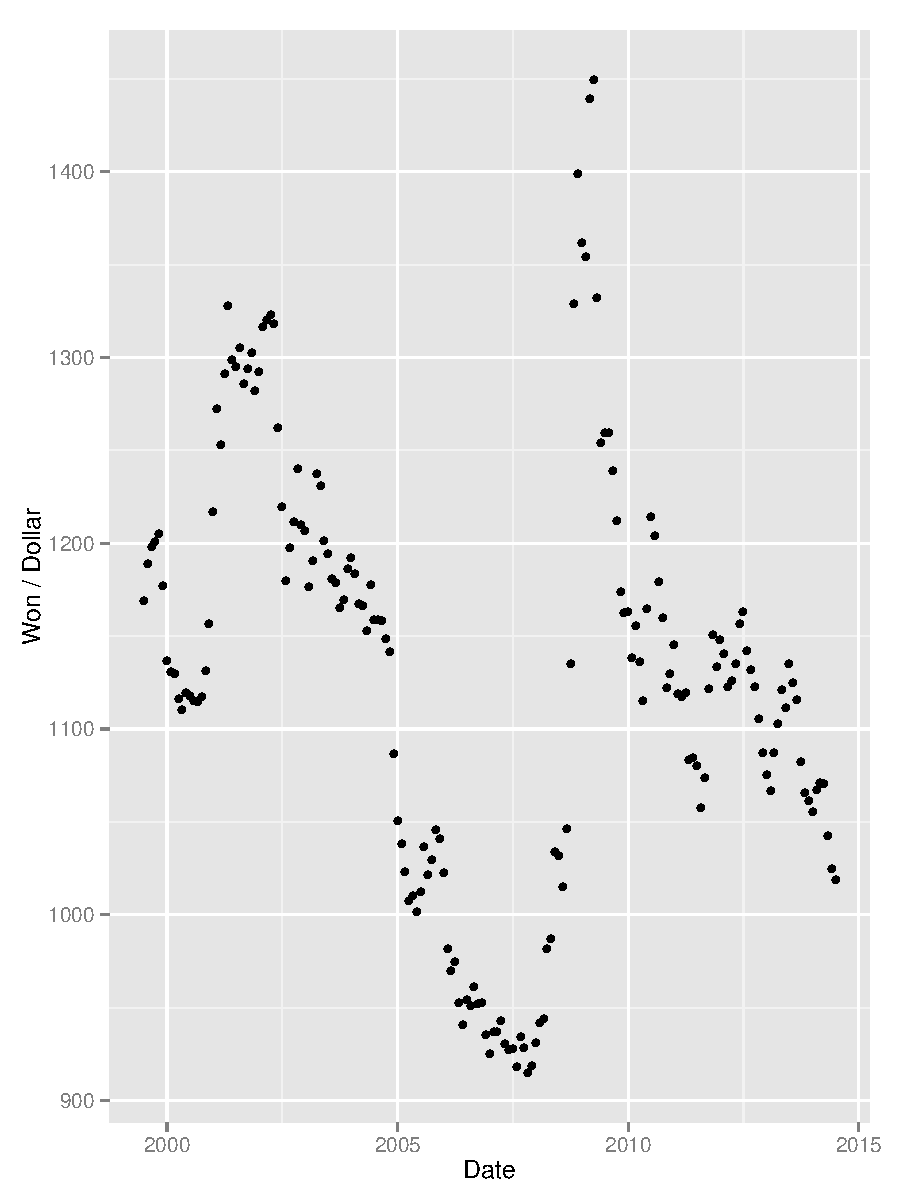
\includegraphics{exchange_rate.pdf}
  \caption{Exchange rate between US and South Korea from 1999 to 2014}
  \label{fig:exchange_rate}
\end{figure}

\begin{figure}
  \centering
    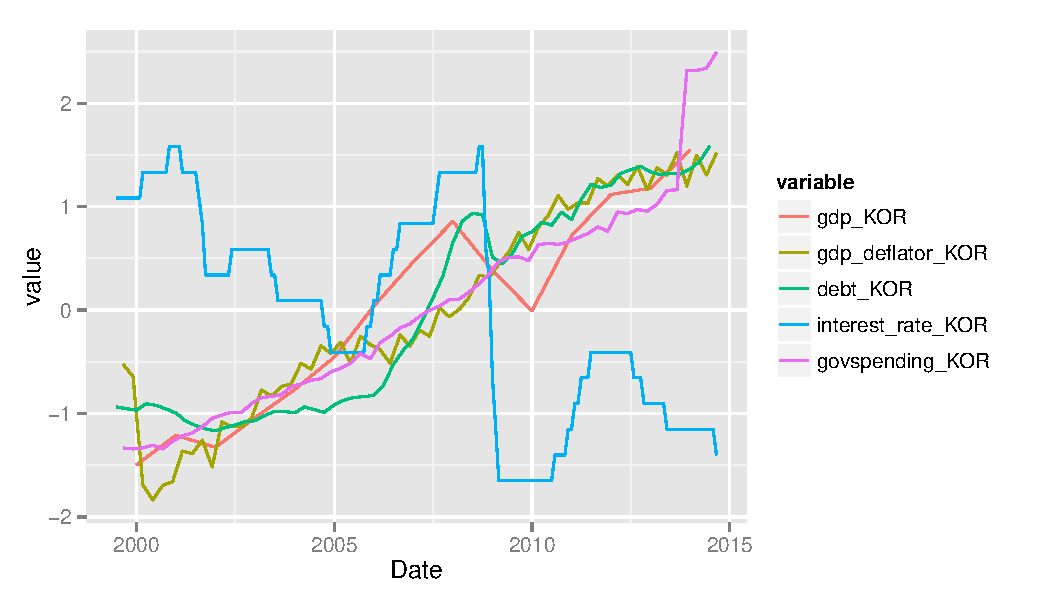
\includegraphics{na_plot_KOR.pdf}
  \caption{Scaled variables with NA values}
  \label{fig:na_plot_KOR}
\end{figure}

\begin{figure}
  \centering
    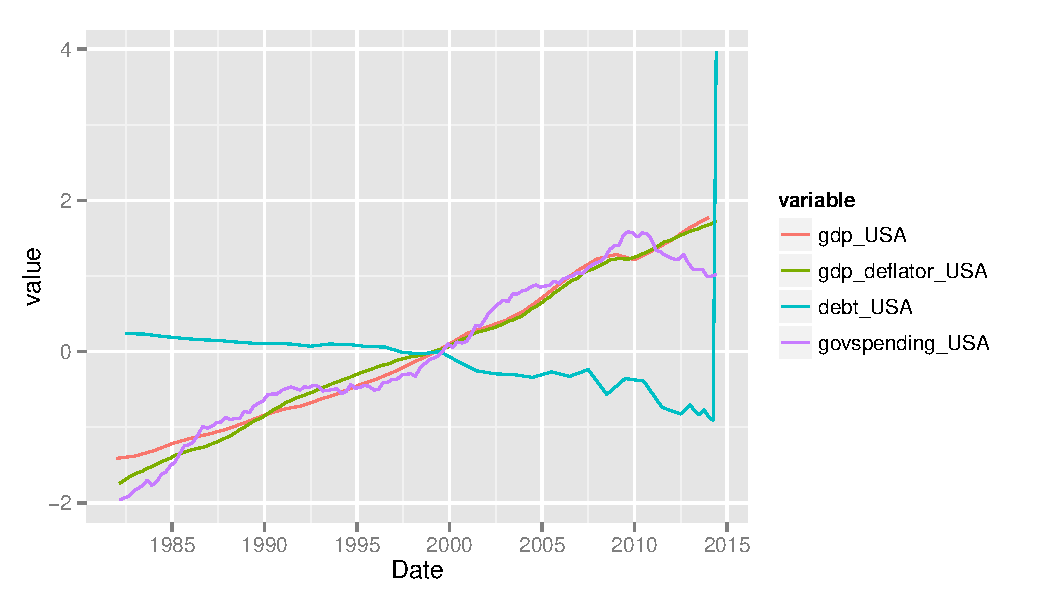
\includegraphics{na_plot_USA.pdf}
  \caption{This figure illustrates the perils of depending on live data. US debt was
formerly measured as a negative number, which is why it was decreasing. But
midway through our analysis the source began to return a huge positive
number for the most recent dates.}

  \label{fig:na_plot_USA}
\end{figure}
\begin{figure}
  \centering
    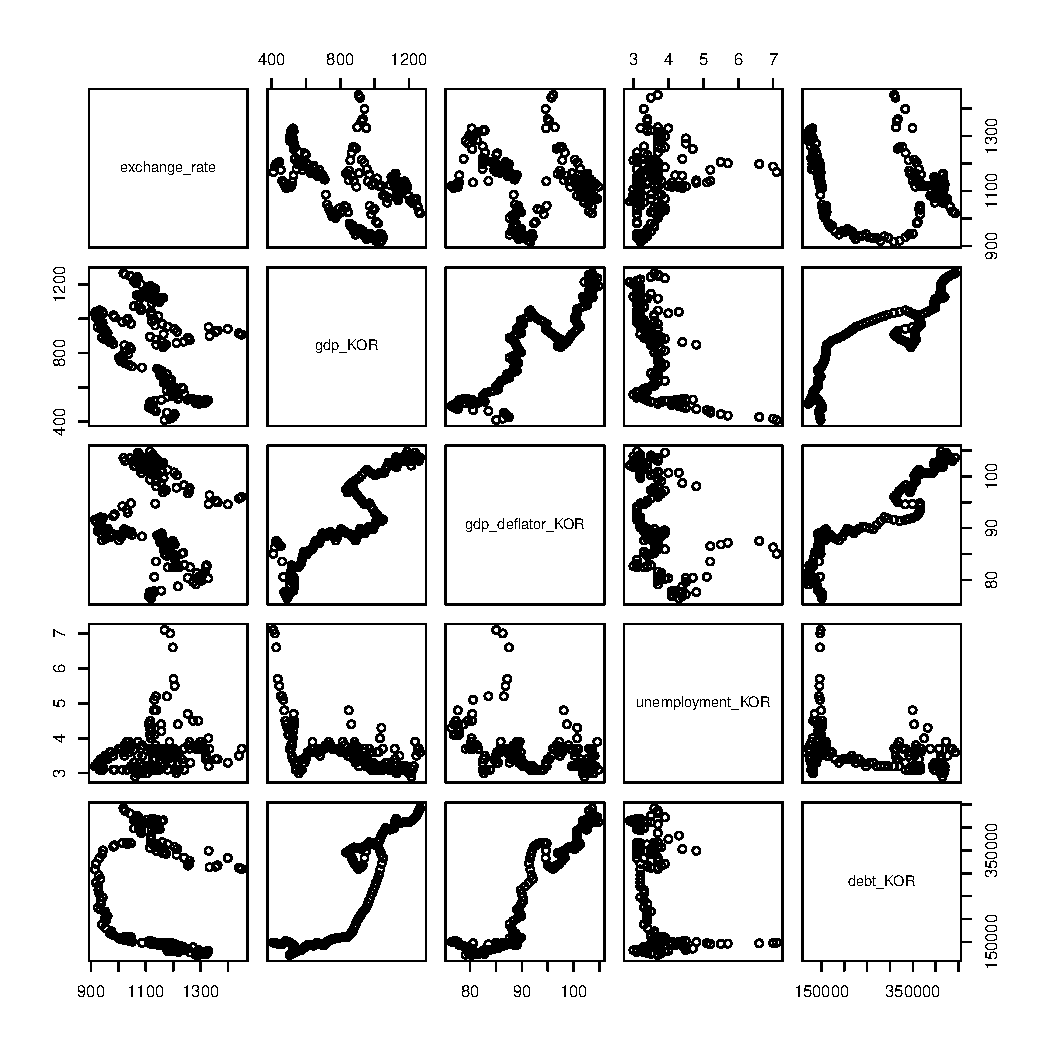
\includegraphics{scatterplot.pdf}
  \caption{Scatterplot of untransformed data}
  \label{fig:scatterplot}
\end{figure}

\begin{figure}
  \centering
    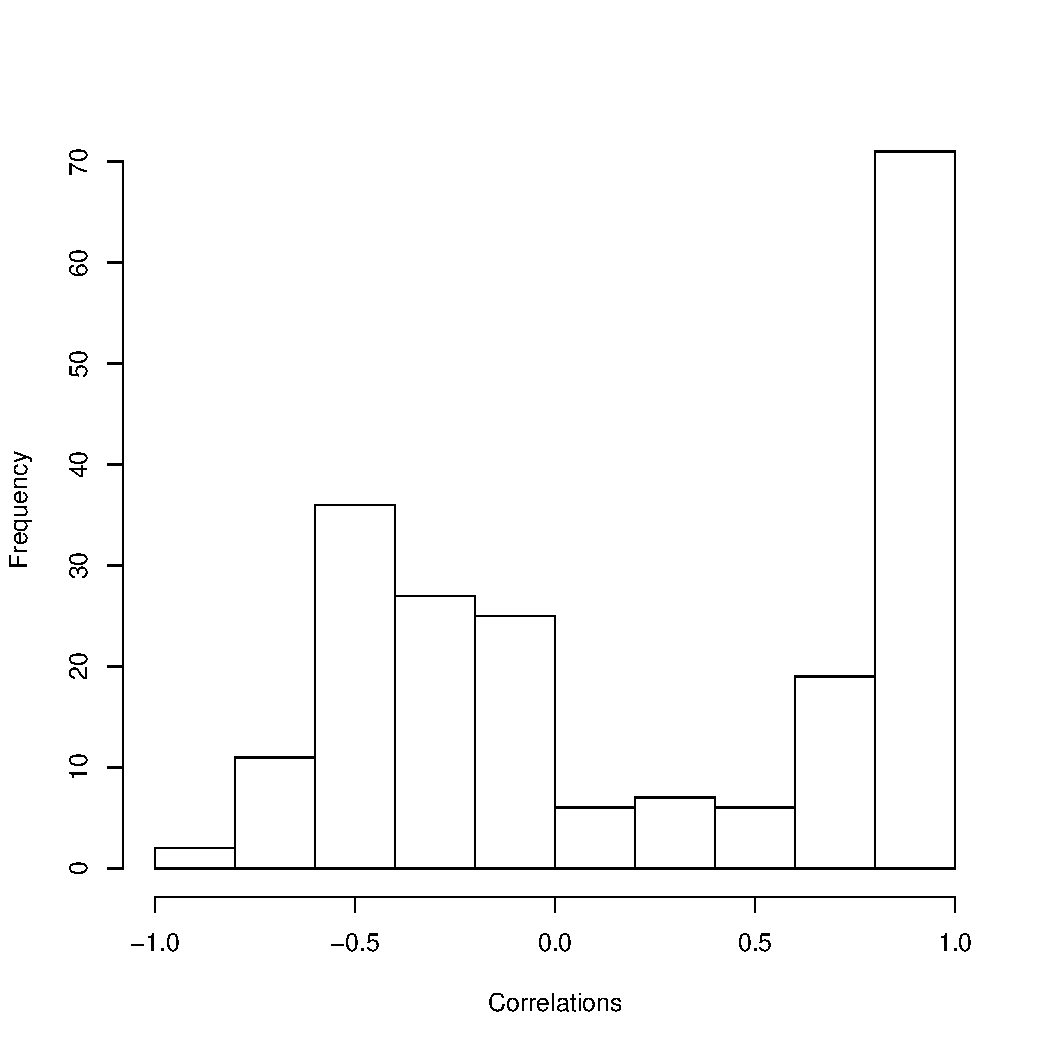
\includegraphics{correlation.pdf}
  \caption{Histogram of all pairwise sample correlations}
  \label{fig:correlation}
\end{figure}

\begin{figure}
  \centering
    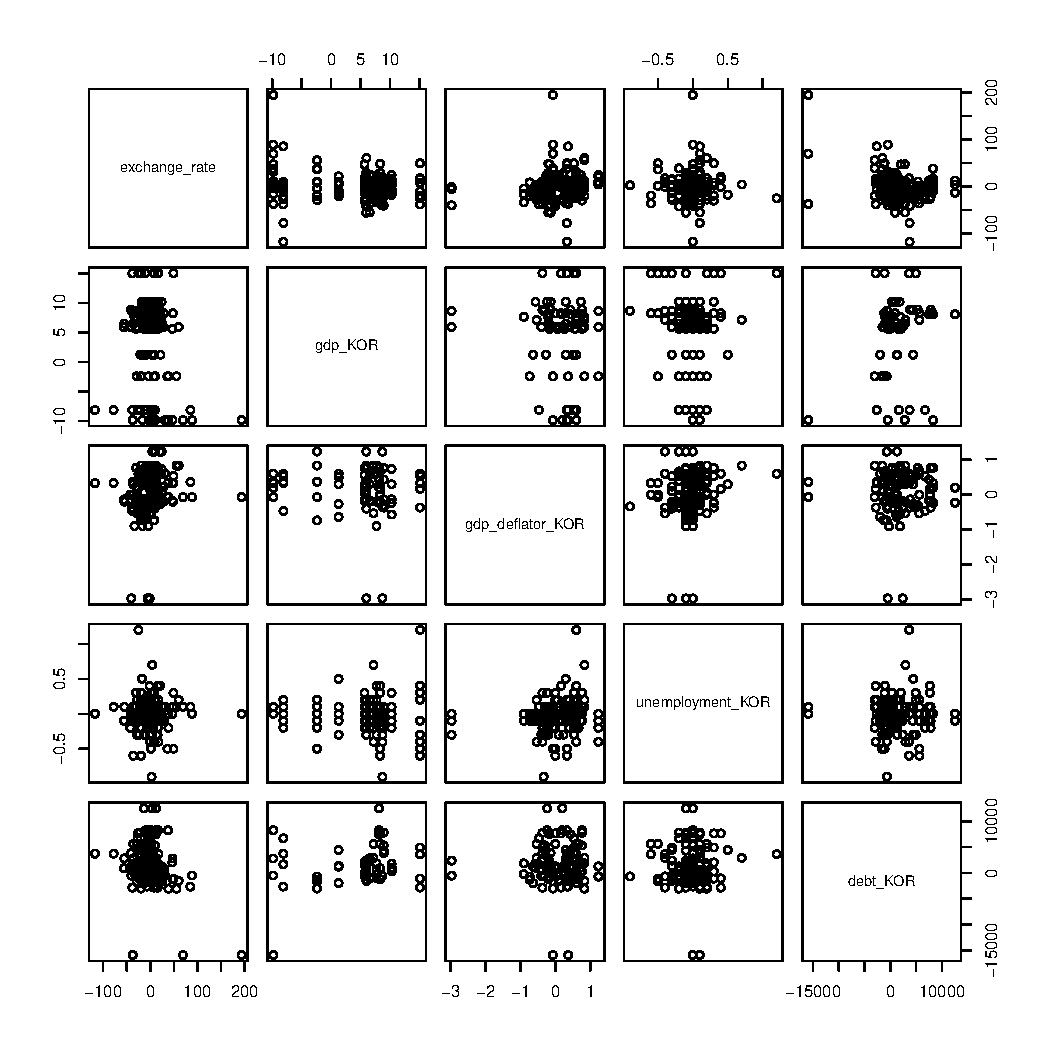
\includegraphics{diff_scatterplot.pdf}
  \caption{Scatterplot of data after row difference transformation}
  \label{fig:diff_scatterplot}
\end{figure}

\begin{figure}
  \centering
    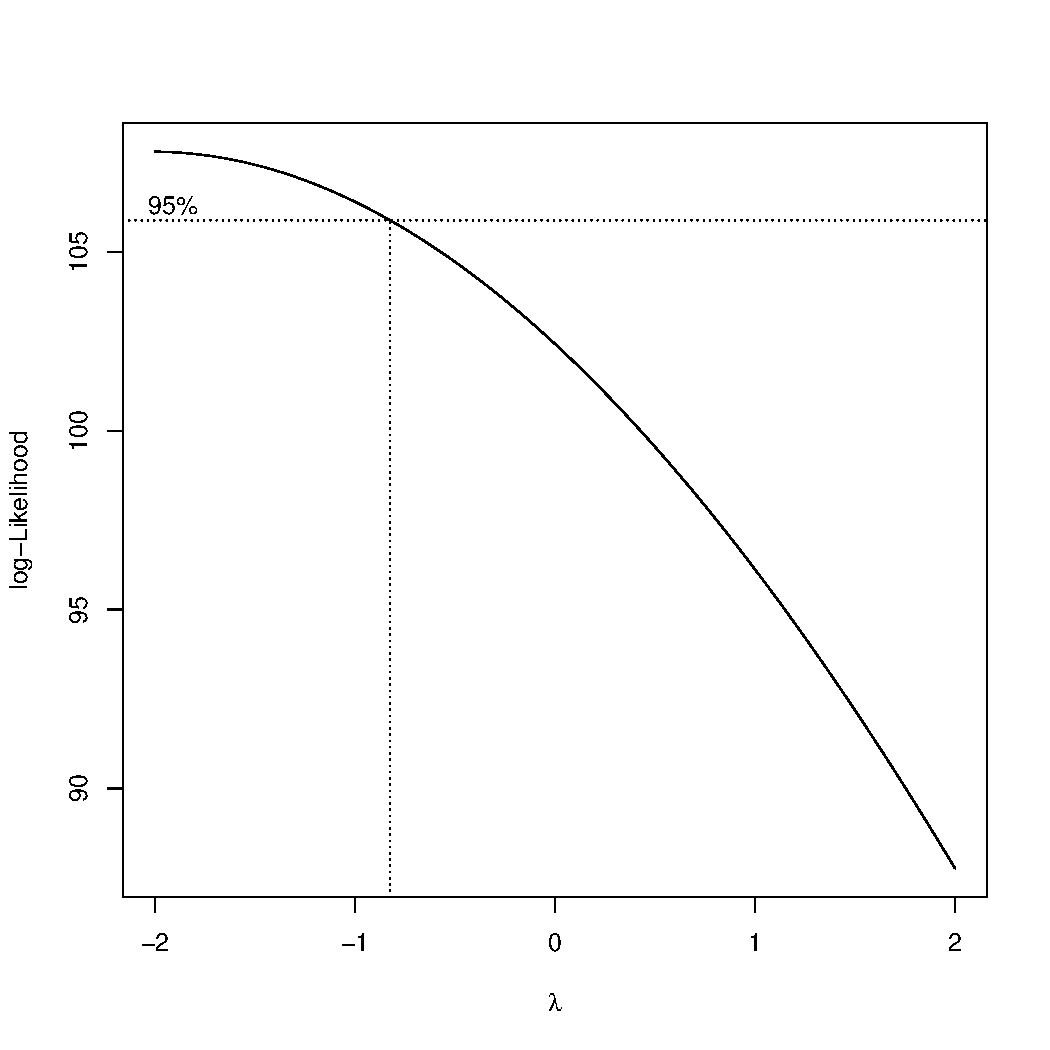
\includegraphics{boxcox.pdf}
  \caption{Box cox procedure on training set- affected by outliers}
  \label{fig:boxcox}
\end{figure}

\begin{figure}
  \centering
    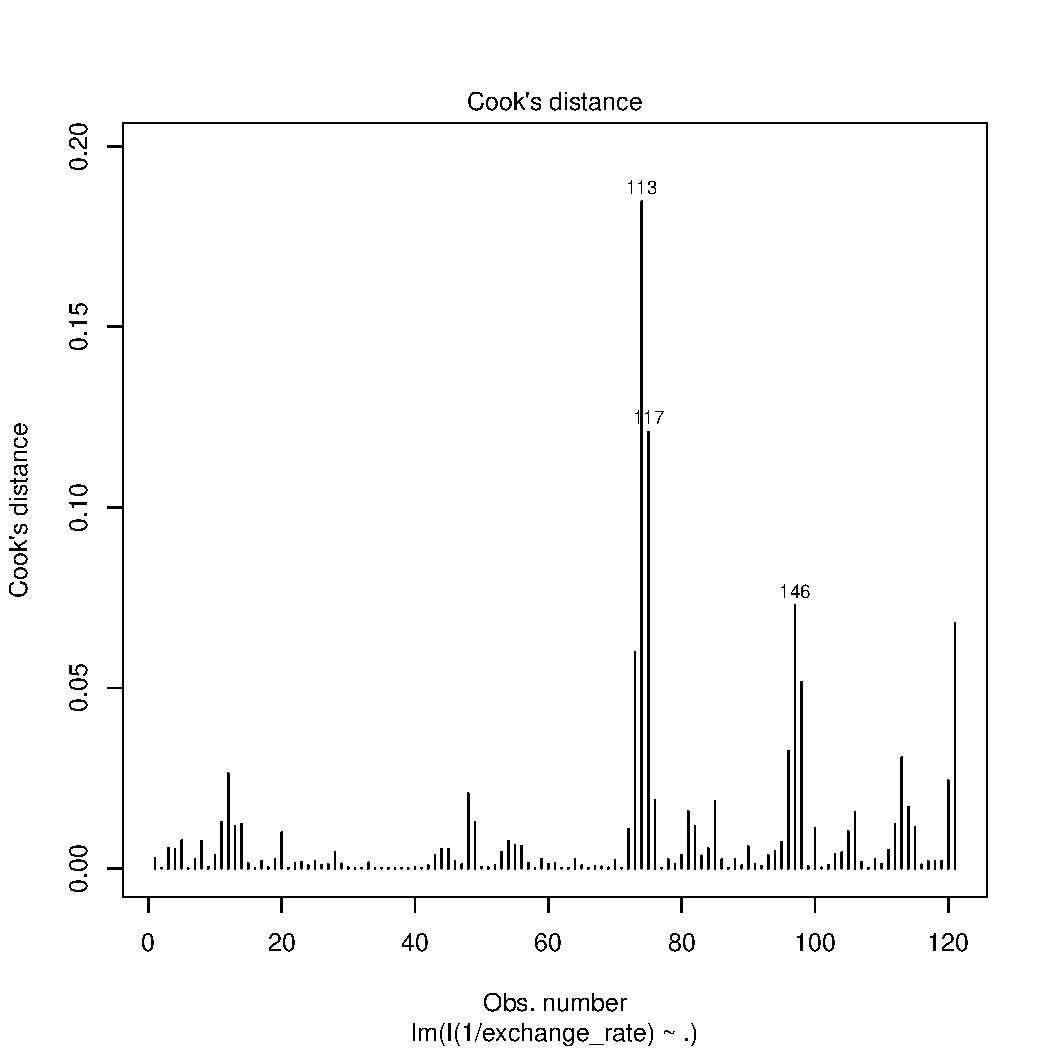
\includegraphics{cooks.pdf}
  \caption{Cooks distance for residuals of training data}
  \label{fig:cooks}
\end{figure}


\begin{figure}
	\centering
	\includegraphics{Addedvariable.pdf}
	\caption{Added-Variable Plot for Government Spending}
	\label{fig:added}
\end{figure}

\begin{figure}
  \centering
    \includegraphics{final_residual.pdf}
  \caption{final residual plots for centered model}
  \label{fig:final_residual}
\end{figure}



\newpage
.
\newpage

\section{Appendix 2 - R Output}

\subsection*{Model Selection Output}
\begin{table}[ht]
	\centering
	\begin{tabular}{rrrrrr}
		\hline
		& sse & bic & r2 & r2a & cp \\
		\hline
		1 & 0.00 & -46.47 & 0.37 & 0.37 & 411.04 \\
		2 & 0.00 & -178.62 & 0.80 & 0.79 & 55.28 \\
		3 & 0.00 & -185.95 & 0.82 & 0.81 & 41.04 \\
		4 & 0.00 & -206.51 & 0.85 & 0.85 & 13.91 \\
		5 & 0.00 & -212.36 & 0.86 & 0.86 & 5.39 \\
		6 & 0.00 & -210.43 & 0.87 & 0.86 & 4.72 \\
		7 & 0.00 & -207.14 & 0.87 & 0.86 & 5.33 \\
		8 & 0.00 & -202.47 & 0.87 & 0.86 & 7.22 \\
		9 & 0.00 & -197.85 & 0.87 & 0.86 & 9.06 \\
		10 & 0.00 & -193.12 & 0.87 & 0.86 & 11.00 \\
		\hline
	\end{tabular}
\end{table}

\subsection{Influence Measures}

\begin{table}[ht]
\centering
\begin{tabular}{rrrrrrrrrrr}
  \hline
 & dfb.1\_ & dfb.gdp & dfb.int\_ & dfb.i\_KO & dfb.i\_US & dfb.gvsp & dffit & cov.r & cook.d & hat \\
  \hline
110 & -0.15 & -0.04 & -0.09 & 0.18 & 0.06 & 0.11 & 0.25 & 1.16 & 0.01 & 0.12 \\
  113 & 0.67 & 0.18 & 0.43 & -0.93 & 0.00 & -0.51 & -1.17 & 0.30 & 0.18 & 0.05 \\
  117 & 0.24 & 0.01 & 0.21 & -0.65 & 0.70 & -0.18 & -0.89 & 0.67 & 0.12 & 0.07 \\
  122 & -0.02 & -0.02 & 0.01 & -0.00 & 0.07 & 0.01 & -0.08 & 1.18 & 0.00 & 0.11 \\
  173 & -0.03 & -0.03 & -0.03 & -0.00 & -0.01 & 0.05 & 0.08 & 1.16 & 0.00 & 0.09 \\
  176 & -0.05 & -0.05 & -0.05 & 0.01 & 0.00 & 0.09 & 0.11 & 1.24 & 0.00 & 0.16 \\
  177 & -0.06 & -0.05 & -0.05 & 0.01 & -0.01 & 0.09 & 0.11 & 1.24 & 0.00 & 0.15 \\
  178 & -0.06 & -0.05 & -0.05 & 0.02 & -0.00 & 0.10 & 0.11 & 1.24 & 0.00 & 0.16 \\
  179 & -0.21 & -0.20 & -0.18 & 0.06 & 0.02 & 0.33 & 0.38 & 1.20 & 0.02 & 0.16 \\
  180 & -0.37 & -0.33 & -0.30 & 0.13 & 0.04 & 0.57 & 0.64 & 1.12 & 0.07 & 0.16 \\
   \hline
\end{tabular}
\end{table}

\subsubsection{Model1 summary output (Train Data)\label{m1:train}}
\begin{verbatim}
Call:
lm(formula = I(1/exchange_rate) ~ ., data = tdata8)

Residuals:
Min         1Q     Median         3Q        Max 
-7.807e-05 -1.661e-05 -3.530e-07  2.128e-05  6.973e-05 

Coefficients:
               Estimate   Std. Error t value Pr(>|t|)    
(Intercept)    3.901e-04  2.851e-05  13.683  < 2e-16 ***
gdp            1.130e-02  5.522e-04  20.471  < 2e-16 ***
interest_rate -1.211e-05  1.085e-06 -11.158  < 2e-16 ***
inflation_KOR -1.877e-05  3.334e-06  -5.630 1.35e-07 ***
inflation_USA  1.529e-05  2.574e-06   5.943 3.23e-08 ***
govspending   -9.170e-06  3.423e-06  -2.679   0.0085 ** 
---
Signif. codes:  0 ‘***’ 0.001 ‘**’ 0.01 ‘*’ 0.05 ‘.’ 0.1 ‘ ’ 1

Residual standard error: 2.863e-05 on 112 degrees of freedom
Multiple R-squared:  0.9034,	Adjusted R-squared:  0.8991 
F-statistic: 209.4 on 5 and 112 DF,  p-value: < 2.2e-16
\end{verbatim}

\subsubsection{Model1 summary output (Validation Data)\label{m1:test}}

\begin{verbatim}
Call:
lm(formula = I(1/exchange_rate) ~ ., data = test99)

Residuals:
Min         1Q     Median         3Q        Max 
-6.962e-05 -1.878e-05 -2.636e-06  1.988e-05  4.937e-05 

Coefficients:
               Estimate   Std. Error t value Pr(>|t|)    
(Intercept)    4.038e-04  3.592e-05  11.244 1.56e-15 ***
gdp            1.001e-02  7.838e-04  12.769  < 2e-16 ***
interest_rate -1.163e-05  1.601e-06  -7.268 1.85e-09 ***
inflation_KOR -2.808e-05  3.749e-06  -7.492 8.15e-10 ***
inflation_USA  2.315e-05  4.847e-06   4.776 1.50e-05 ***
govspending   -3.640e-06  4.246e-06  -0.857    0.395    
---
Signif. codes:  0 ‘***’ 0.001 ‘**’ 0.01 ‘*’ 0.05 ‘.’ 0.1 ‘ ’ 1

Residual standard error: 2.742e-05 on 52 degrees of freedom
Multiple R-squared:  0.9161,	Adjusted R-squared:  0.908 
F-statistic: 113.5 on 5 and 52 DF,  p-value: < 2.2e-16
\end{verbatim}


\subsubsection{Summary table of Final model}

\label{finalmodel}
\begin{verbatim}
Call:
lm(formula = I(1/exchange_rate) ~ gdp + interest_rate + inflation_KOR + 
inflation_USA, data = alldata)

Residuals:
Min         1Q     Median         3Q        Max 
-1.631e-04 -1.924e-05  4.079e-06  2.177e-05  8.537e-05 

Coefficients:
               Estimate   Std. Error t value Pr(>|t|)    
(Intercept)    3.868e-04  2.285e-05  16.929  < 2e-16 ***
gdp            9.692e-03  4.007e-04  24.190  < 2e-16 ***
interest_rate -1.289e-05  8.636e-07 -14.927  < 2e-16 ***
inflation_KOR -2.573e-05  2.637e-06  -9.758  < 2e-16 ***
inflation_USA  2.136e-05  2.646e-06   8.072 1.04e-13 ***
---
Signif. codes:  0 ‘***’ 0.001 ‘**’ 0.01 ‘*’ 0.05 ‘.’ 0.1 ‘ ’ 1

Residual standard error: 3.58e-05 on 176 degrees of freedom
Multiple R-squared:  0.8555,	Adjusted R-squared:  0.8522 
F-statistic: 260.5 on 4 and 176 DF,  p-value: < 2.2e-16
\end{verbatim}

\subsubsection{Final model Summary Output(Centered data)}
\label{centered}

\begin{verbatim}
Call:
lm(formula = exchange_rate ~ gdp + exports + interest_rate + 
inflation_KOR + inflation_USA, data = sdata_n)

Residuals:
Min       1Q   Median       3Q      Max 
-0.72512 -0.22635  0.00475  0.16783  0.94453 

Coefficients:
              Estimate    Std. Error t value Pr(>|t|)    
(Intercept)   -0.03923    0.02417  -1.623    0.106    
gdp           -0.68565    0.04872 -14.073  < 2e-16 ***
exports       -0.24752    0.05083  -4.869 2.54e-06 ***
interest_rate  0.59072    0.03611  16.361  < 2e-16 ***
inflation_KOR  0.28550    0.02762  10.337  < 2e-16 ***
inflation_USA -0.29924    0.03197  -9.361  < 2e-16 ***
---
Signif. codes:  0 ‘***’ 0.001 ‘**’ 0.01 ‘*’ 0.05 ‘.’ 0.1 ‘ ’ 1

Residual standard error: 0.3211 on 171 degrees of freedom
Multiple R-squared:  0.8868,	Adjusted R-squared:  0.8835 
F-statistic: 267.9 on 5 and 171 DF,  p-value: < 2.2e-16
\end{verbatim}

\section{Appendix 3 - Reproducibility}

Above we mentioned that the data and all analysis in the report is self 
updating. This is accomplished through the use of GNU \texttt{make}, which
describes a DAG (Directed Acyclic Graph) of dependencies for the final
report. \texttt{make} detects file modifications and will lazily run all
commands and scripts required for the final output.

What does this mean? Suppose that we need more variables to do the
regression. Thanks to the use
of industry standard ISO codes for the countries and proper parameters in
our code base this becomes a simple task.
We've stored string templates for the country level 
variables in a file
called \texttt{template.txt}. The data collection and preprocessing steps
are automated, so we can add more variables simply by adding a row to
\texttt{template.txt} and entering the command \texttt{make} from the shell
prompt, which causes the following sequence of events: 

\begin{enumerate}
    \item \texttt{make} detects the changed template file
    \item The script \texttt{download.R} runs, updating the cache
    \item The script \texttt{preprocess.R} runs, applying the appropriate
        transformations and joining the tables to a form suitable for
        analysis
    \item All other scripts which depend on the preprocessed data run
    \item The report output is produced
\end{enumerate}

In this case the output is a PDF, but it could just as easily be a web page
on the department server, or an upload into another REST API.

If we were doing this analysis for a client and need to run it again a year
later with a new year of data 
then all we have to do is type \texttt{make}. We'll still need to interpret
plots and models, but the most time consuming work is done.

One other aspect of reproducibility is version control. In this
project we've used \texttt{Git} to collect snapshots of the project at
every stage. The project is hosted publicly on
Github\footnote{\url{https://github.com/clarkfitzg/stats206\_project}}.
A look at the log file shows what work happened when and why,
which is important for establishing provenance. In particular it shows 
that we've been active on this project every day since
December 1st, pushed more than 30 commits, and wrote nearly 3000 lines of
code (including \LaTeX). Here's an example of a log entry:

\begin{verbatim}
commit e2beaf01b0a1457e7167989c1fae575c2a676f19
Author: Clark Fitzgerald <clarkfitzg@gmail.com>
Date:   Mon Dec 8 20:51:04 2014 -0800

    implemented local caching, decoupled download step
\end{verbatim}

Through a little engineering the data analysis process
can be made transparent, automated, extensible, and fully reproducible.


\end{document}
